\chapter{Resultate}
\label{ch_resultat}

Im Kapitel \ref{ch_vorgehen} ist die Umsetzung ausführlich erklärt. In diesem Kapitel geht es um die relevanten Resultate. Diese teilen sich in die bekannten Kategorien Harvester, Energy - und Power Management sowie die BLE-Applikation. Die Resultate jeder Kategorie werden in einem Unterkapitel beschrieben.
 
\section{Harvesterschaltung}

\subsection{Der Print}

Die erstellte Leiterplatte ist in den Abbildungen \ref{print_vorne} und \ref{print_rueckseite} zusehen. Auf der Ansicht von oben ist der Top-Layer inklusive der Bestückung zu sehen. Die Bestückung des Top-Layers beinhaltet die Harvesterschaltung (unten rechts), den EM8500 (oben rechts) und den Stecker (mittig links), welcher als Verbindung zum TI-SensorTag dient. Ebenfalls sind die vielen Testpunkte zu sehen, jedes Netz wurde mit einem Testpunkt ausgestattet. Oben links sind die Anschlüsse für die Energiespeicher zu sehen, hier wurden die beiden Kondensatoren über Litzen angeschlossen, da die Elkos keinen Platz zwischen dem Prototypen-PCB und dem TI-SensorTag finden. 

Auf der Ansicht von unten ist der Bottom-Layer inklusive der Bestückung zu sehen. Die Unterseite der Leiterplatte beherrbergt die Spule und den Reed-Switch, welche auf der oberen Seite der Leiterplatte keinen Platz mehr gefunden haben. Der Reed-Switch hätte vielleicht noch Platz gehabt auf der oberen Seite, jedoch muss der Reed-Switch in der Nähe der Spule paltziert werden, da hier der Magnet durchläuft.

\begin{figure}[ht]
    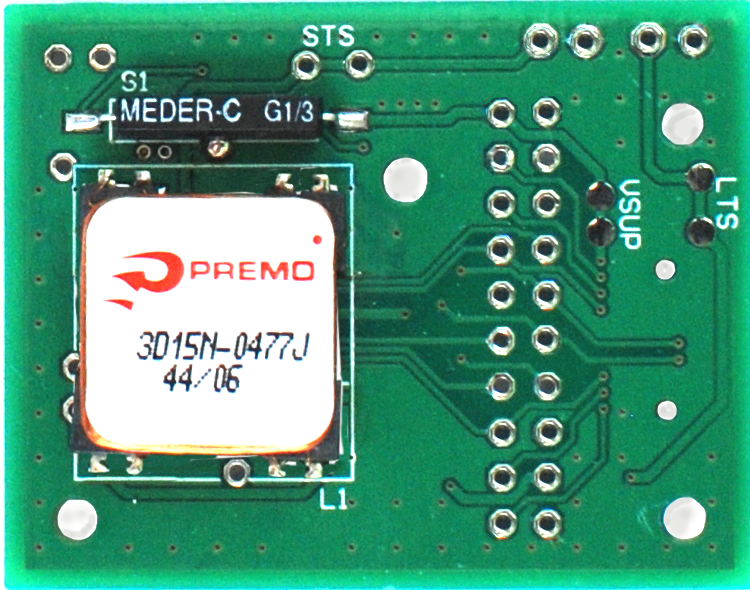
\includegraphics[width=0.5\textwidth]{4Resultate/imag/print_rueckseite.png} 
    \caption{Print Ansicht von unten}
    \label{print_rueckseite}
\end{figure}


\begin{figure}[ht]
    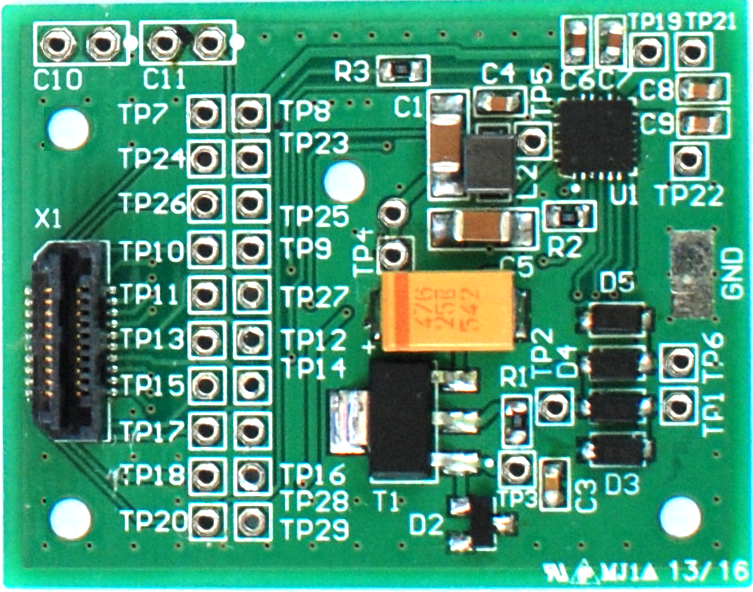
\includegraphics[width=0.5\textwidth]{4Resultate/imag/print_vorne.png} 
    \caption{Print Ansicht von oben}
    \label{print_vorne}
\end{figure}

\newpage  % todel
\subsection{Leistung am Harvesterausgang}

Wie erwartet (siehe theoretische Grundlagen \ref{mpp_theorie_diff}) ändert sich bei einer Hardware mit einer Spule das Leistungsmaximum. Die Abbildung \ref{mpp_resultat_harvester} zeigt die reale MPP-Kurve des Prototypen. Bei verschiedenen Geschwindigkeiten ist der MPP an einem anderen Punkt, problematisch ist, dass die Einstellung im EM8500 nicht so genau eingestellt werden kann, es sind nur grobe Schritte im Bereich von 50 - 70 \% verfügbar. 

\begin{figure}[ht]
    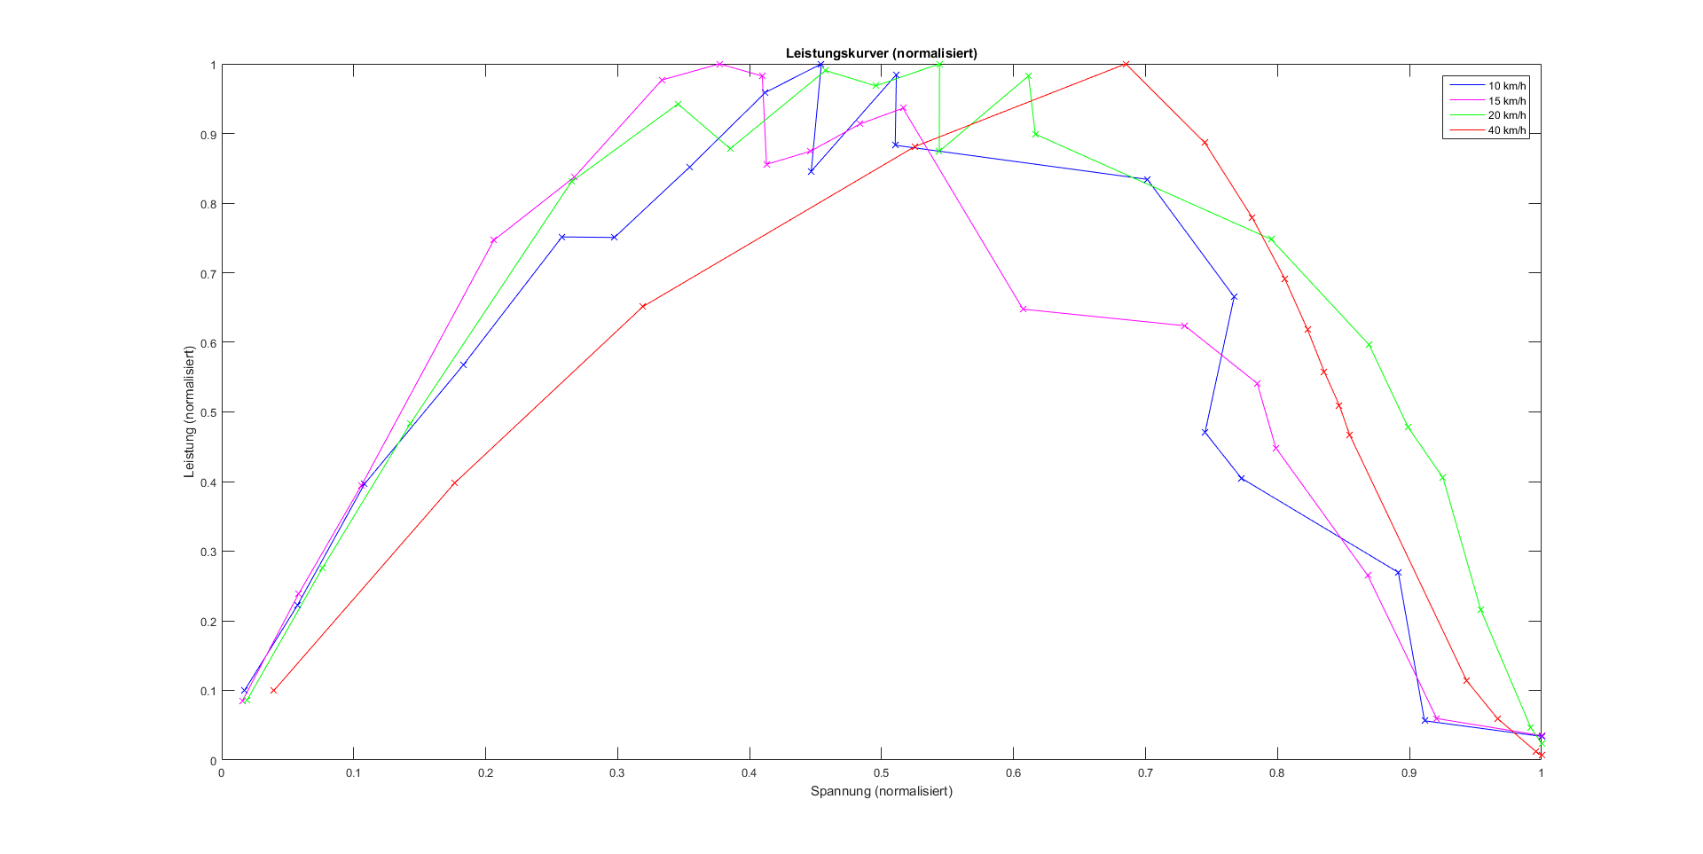
\includegraphics[width=0.5\textwidth]{4Resultate/imag/MPPHarvester.png} 
    \caption{Leistungskurve Harvesterausgang (normalisiert)}
    \label{mpp_resultat_harvester}
\end{figure}

Die Leistung, welche der Harvester zur Verfügung stellen kann liegt bereits bei einer Geschwindigkeit von 10 km/h bei 24.77 $\mu$W. Dies ist die Durchschnittsleistung bei optimaler Belastung, es handelt sich nicht um die Spitzenleistung. Es ist ersichtlich dass die Leistung mit der steigender Geschwindigkeit zunimmt.

\begin{tabbing}
    Geschwindigkeit \quad\= Leistung Harvester \\[0.8ex]
    10 km/h  \> 24.77  $\mu$W \\
    15 km/h  \> 61.07  $\mu$W \\
    20 km/h> \> 116.69 $\mu$W \\
    40 km/h> \> 472.61 $\mu$W \\
\end{tabbing}  

Es ist zu beachten, dass diese Werte die Leistung des MPP sind, somit können diese Leistungen nur erreicht werden, wenn die Einstellung des EM8500-Chips dementsprechend eingestellt werden.


\newpage  % todel
\subsection{Verhalten des Harvesterausgangs}

Die Abbildung \ref{resultat_Harvester_Spannung_47uF} zeigt das Verhalten des Harvesterausgangs mit einem 47 $\mu$F Elko bei der Belastung durch den EM8500-Chip. Die Spannung ist über einen längeren Zeitraum betrachtet sehr instabil, diese Problematik wurde bereits im Kapitel \ref{Ausmessen der Auswirkung des Ausgangskondensators} beschrieben. Die Abbildung \ref{resultat_Harvester_Spannung_100uF} zeigt das reelle Verhalten des Harvesterausgangs mit einem 100 $\mu$F Elko. Es ist zu sehen, dass die Spannung am Harvesterausgang über einen längeren Zeitraum relativ konstant bleibt. Genaue Messdaten zu dieser Problematik sind im Messprotokoll \todo{Messprotokoll} zu finden.

\begin{figure}[ht]
    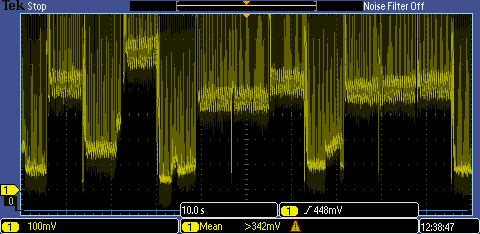
\includegraphics[width=0.5\textwidth]{4Resultate/imag/SpannungVCC_47uF.png} 
    \caption{Spannung VCC beim Harvesterausgang bei 15 km/h}
    \label{resultat_Harvester_Spannung_47uF}
\end{figure}

\begin{figure}[ht]
    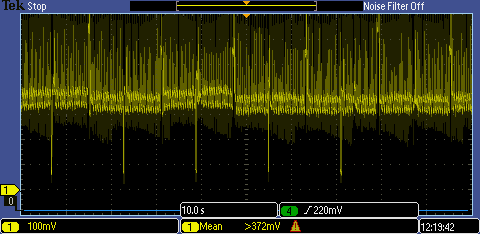
\includegraphics[width=0.5\textwidth]{4Resultate/imag/SpannungVCC_100uF.png} 
    \caption{Spannung VCC beim Harvesterausgang bei 15 km/h}
    \label{resultat_Harvester_Spannung_100uF}
\end{figure}

\newpage  % todel
\subsection{Energie am EM-Chipausgang}

Die Abbildung \ref{energie_resultat_harvester} zeigt die berechnete Energie, die am Ausgang des EM-Chip abgegeben wird in Bezug zur Geschwindigkeit. Die Berechnung, wie aus dem Puls über die Zeit, bis dass VSUP wieder eingeschalten wird, ist im  Messprotokoll yyy dokumentiert. Die gewonnene Energie, die dem TI-SensorTag zur Verfügung steht ist:

\subsubsection*{Tabelle Leistung und Wirkungsgrad }
\begin{tabbing}
    Geschwindigkeit \quad\= Leistung EM8500\_out \\[0.8ex]
    10 km/h  \> 5.44   $\mu$W\\
    15 km/h  \> 20.91  $\mu$W\\
    20 km/h> \> 41.39  $\mu$W\\
    40 km/h> \> 170.75 $\mu$W\\
\end{tabbing}  


\begin{figure}[ht]
    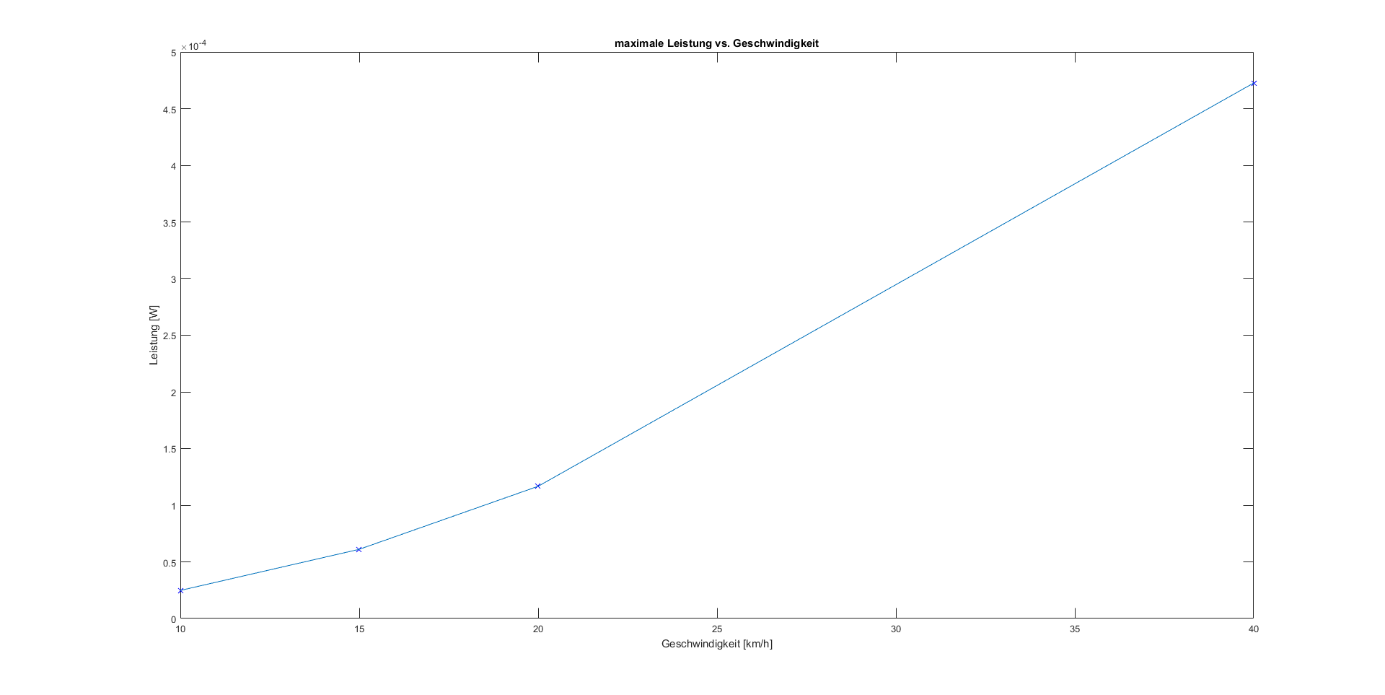
\includegraphics[width=0.5\textwidth]{4Resultate/imag/ResultatLeistungGeschwindigkeit.png} 
    \caption{Maximale Leistung vs. Geschwindigkeit}
    \label{energie_resultat_harvester}
\end{figure}

\subsection{Wirkungsgrad des Prototypen}

Aus den zwei Leistungsmessungen wird graphisch die Energiegewinnung im Vergleich dargestellt (Abbildung \ref{zsmEnergyGewinn}). Die Werte beziehen sich auf die gemittelte Leistung über 10 s. Es ist zu sehen, dass die Energiegewinnung bei der Harvesterschaltung mit der Geschwindigkeit deutlich schneller zunimmt, als die Energie am Ausgang des EM-Chips. 

\begin{figure}[ht]
    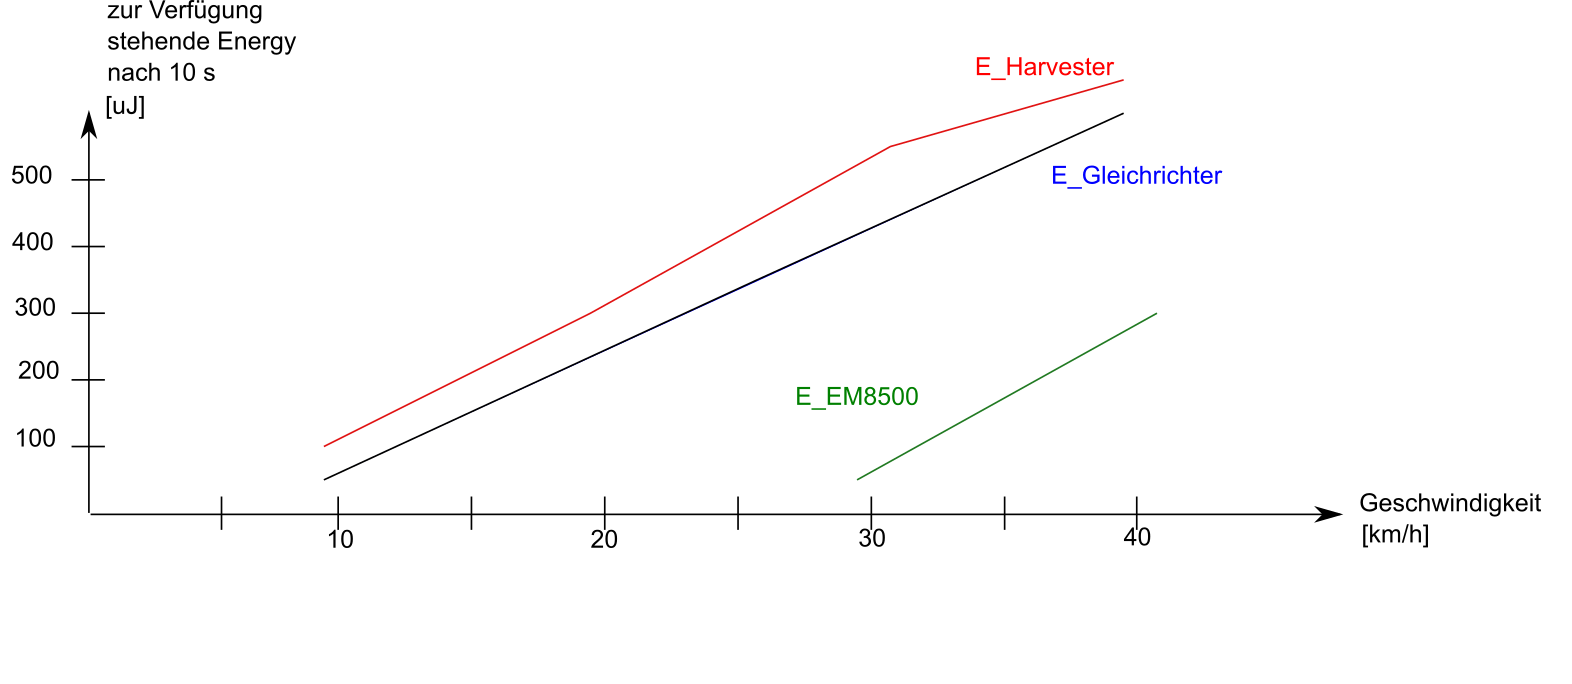
\includegraphics[width=1\textwidth]{4Resultate/imag/EnergyGewinnNachStelle.png} 
    \caption{Energiegewinn Zusammengefasst nach Stelle in der Schaltung}
    \label{zsmEnergyGewinn}
\end{figure}

Aus den zwei Leistungsmessungen wurde der Wirkungsgrad bei den gemessenen Geschwindigkeiten berechnet (siehe Tabelle unten). Der Wirkungsgrad ist bei tiefen Geschwindigkeiten sehr schlecht (24.87\thinspace\%). Dies ist eine der zwei Ursache, dass trotz genug geernteter Energie, das TI-SensorTag für das Senden der Sensorwerte bei tiefer Geschwindigkeiten nicht wie erwartet genug Energie hat. Mit mehr Geschwindigkeit, erhöht sich nicht nur die geerntete Leistung rapide, sondern auch der Wirkungsgrad. Der Wirkungsgrad des EM8500 innerhalb des entwickelten Prototypen liegt bei 40 km/h  bei 41.01\thinspace\%.  

\subsubsection*{Tabelle Leistung und Wirkungsgrad }
\begin{tabbing}
    Geschwindigkeit \quad\= Leistung Harvester \quad\= Leistung EM8500\_out \quad\= Wirkungsgrad\\[0.8ex]
    10 km/h  \> 21.87  $\mu$W \> 5.44   $\mu$W \> 24.87\thinspace\%  \\
    15 km/h  \> 57.19  $\mu$W \> 20.91  $\mu$W \> 36.56\thinspace\%  \\
    20 km/h \> 114.67 $\mu$W \> 41.39  $\mu$W \> 36.09\thinspace\%  \\
    40 km/h \> 416.29 $\mu$W \> 170.75 $\mu$W \> 41.01\thinspace\%  \\
\end{tabbing}   



\section{Energy Management}

%Beim Resultat spielt das Hard- und Softwaremanagment direkt ineinander, weshalb das Ergebnisse dieser zwei Aufgaben zusammen dargestellt werden.

Das Ziel beim Energy Management ist, dass die vom Long Time Storage gespeicherte Energie für das Versenden der BLE-Pakete genutzt wird. Dies ist (siehe Abbildung \ref{LTSladet}) möglich. Die gesammelte Energie beider Kondensatoren wird für das Sender der BLE-Pakete verwendet. Die benutzten Kondensatorenwerte sind:

STS = 100 $\mu$F

LTS = 2200 $\mu$F

Die Werte ergaben sich aus folgender Energiekalkulation
\begin{equation}
W=\frac{1}{2}\cdot 100 uF \cdot (3.6 - 2.2 V)^{2}=xxxxx uW\label{eq:Energie STS}
\end{equation}

\begin{equation}
W=\frac{1}{2}\cdot 2.2 mF \cdot (3.6 - 2.2 V)^{2}=xxxxx mW\label{eq:Energie LTS}
\end{equation}


Dadurch sammelt STS in einer Periode von xx ms eine Enegrigemenge von \todo{finale Zeiten eintragen. Energie dafür eintragen} yyy mJ. LTS lädt in der Periode von  zz ms zusätzlich eine Energiemenge von yyy mJ. Die angereicherte Menge von tt mJ genügen, um ein xxx-Paket zu versenden.

\todo{besseres Bild}

\begin{figure}[ht]
    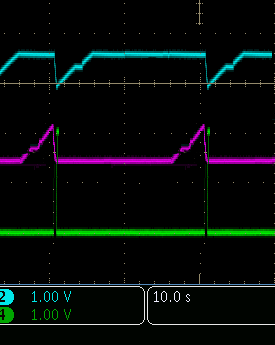
\includegraphics[width=0.5\textwidth]{4Resultate/imag/FakeLTSEntaden.png} 
    \caption{LTS liefert Energie für die Arbeitspakete}
    \label{LTSladet}
\end{figure}

Gelungen ist das Laden und Entladen beider Kondensatoren durch folgende EM-Schwellwerte:

\todo{correct space in table}
% Values from V1
\subsubsection*{Tabelle Finale Konfiguration Schwellwerte }
\begin{tabbing}
    Register .............\quad\= Spannungswert \\[0.8ex]
    v\_bat\_max\_hi       \> 3.9 V \\
    v\_bat\_max\_lo       \> 3.8 V \\
    v\_bat\_min\_hi\_dis  \> 3.6 V \\
    v\_bat\_min\_hi\_con  \> 2.2 V \\
    v\_bat\_min\_lo       \> 2.0 V \\
    v\_appl\_max\_hi      \> 3.8 V \\
    v\_appl\_max\_lo      \> 3.7 V \\   
\end{tabbing}  

\todo{bat mi ni low wird höher}

\section{Powermanagement}

Lange schien es so, dass die Sensoren, aufgrund des grossen Verbrauchs der I2C-Kommunikation und der langen Aufstartzeit der Sensoren, nicht per BLE bei tiefer Geschwindigkeit gesendet werden können. Eine Lösung wurde möglich, weil Aufgabenblöcke in Unterblöcke mit Schlafensezeiten eingebaut wurden. Die untenstehende Tabelle zeit die gefunden Lösung:

\subsubsection*{Tabelle Energieverbrauch Aufgabenblöcke}
\begin{tabbing}
    Funktion ...................................................................................\quad\= Energieverbrauch \\[0.8ex]
    Auslesen Reed Switch und Berechnen Geschwindigkeit       \> xx mW \\
    Starten und Auslesen Drucksensor          \> xx mW \\
    Starten und Auslesen Temperatursensor     \> xx mW \\
    Starten und Auslesen Feuchtigkeitssensor  \> xx mW \\
    Auslesen Statusregister per SPI           \> xx mW \\
\end{tabbing}  


Die Lösung ist das Aufsplitten von Aufgabenblöcken. Bei genug Energie, wird nicht ein Sensor gestartet, ausgelesen und seine Daten versendet, sondern der Sensor wird gestartet, dann geht das System schlafen, bis dass LTS voll ist. Dann folgt der nächste Aufgabe: die Werte auslesen. Es wird wieder geschlafen und beim dritten Mal genügend Energie wird das Paket versendet. Das Konzept des Schlaffens zwischen Aufgabeblöcken ist im theoretischen Teil im Unterkapitel \ref{pm_sleep} im Abschnitt \ref{schlafen_theorie} beschrieben . Die Abbildung \ref{arbeitsaufteilung} zeigt, das Aufteilen der Arbeitsschritte: Zuerst folgt die Initialisierung des Sensors, dann folgt das Auslesen der Daten und zum Schluss das Senden der Werte.

\todo{Bild Arbeitsaufteilung }
\begin{figure}[ht]
    
\includegraphics[width=0.4\textwidth]{idle.png}
    %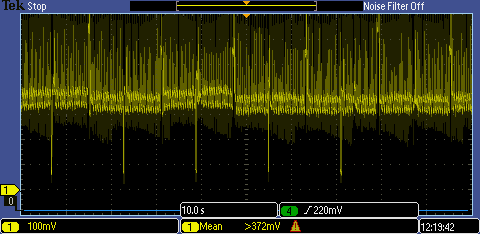
\includegraphics[width=0.1\textwidth]{4Resultate/imag/SpannungVCC.png} 
    \caption{Aufteilen in drei Schritte bis zum Senden der Daten}
    \label{arbeitsaufteilung}
\end{figure}

% ev. Grossaufnahme: BLE Energieverbrauch

Das Ergebnis ist in der Abbildung \ref{Sensor_Energie} graphisch dargestellt. Es zeigt sich, dass das Senden von Sensordaten \todo{Wert eintragen Tabelle und Text} xx mal mehr Energie verbrauchen, als das Senden der Geschwindigkeit. Die schlechteste Bilanz hat das Auslesen des Status Registers aus dem EM8500-Chip. In diesem Byte ist hinterlegt, welche Schwellwerte des EM8500 überschritten wurden und dient dadurch auf einfache Art dem Abbilden des aktuellen Energiezustands (siehe Unterkapitel \ref{v_energiezustand}). 

\begin{figure}[ht]
    
\includegraphics[width=0.4\textwidth]{idle.png}
    %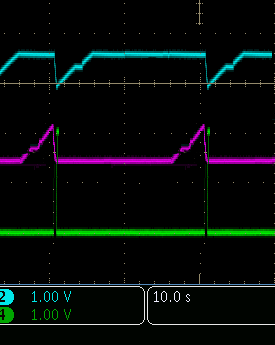
\includegraphics[width=0.5\textwidth]{4Resultate/imag/FakeLTSEntaden.png} 
    \caption{LTS liefert Energie für die Arbeitspakete}
    \label{Sensor_Energie}
\end{figure}


Kombiniert man den Energieverbrauch mit der zur Verfügung stehenden Energie am Ausgang nach dem EM8500-Chips, können (siehe Abbildung \ref{resultat_Zsm_Energy}) folgende Schlussfolgerungen gezogen werden:

\todo{ genauere Angaben nach Endmessungen}
\begin{enumerate}
    \item Das Übermitteln der Geschwindigkeit ist ab 10 km/h möglich
    \item Das Übermitteln aller Sensordaten (gestaffelt) ist ab xxx km/h möglich
    \item Das Übermitteln aller Sensordaten braucht bei einer Geschwindigkeit von 10 km/h xxxx s
    \item Das Übermitteln aller Sensordaten braucht bei 40 km/h xxx s
\end{enumerate}

\begin{figure}[ht]
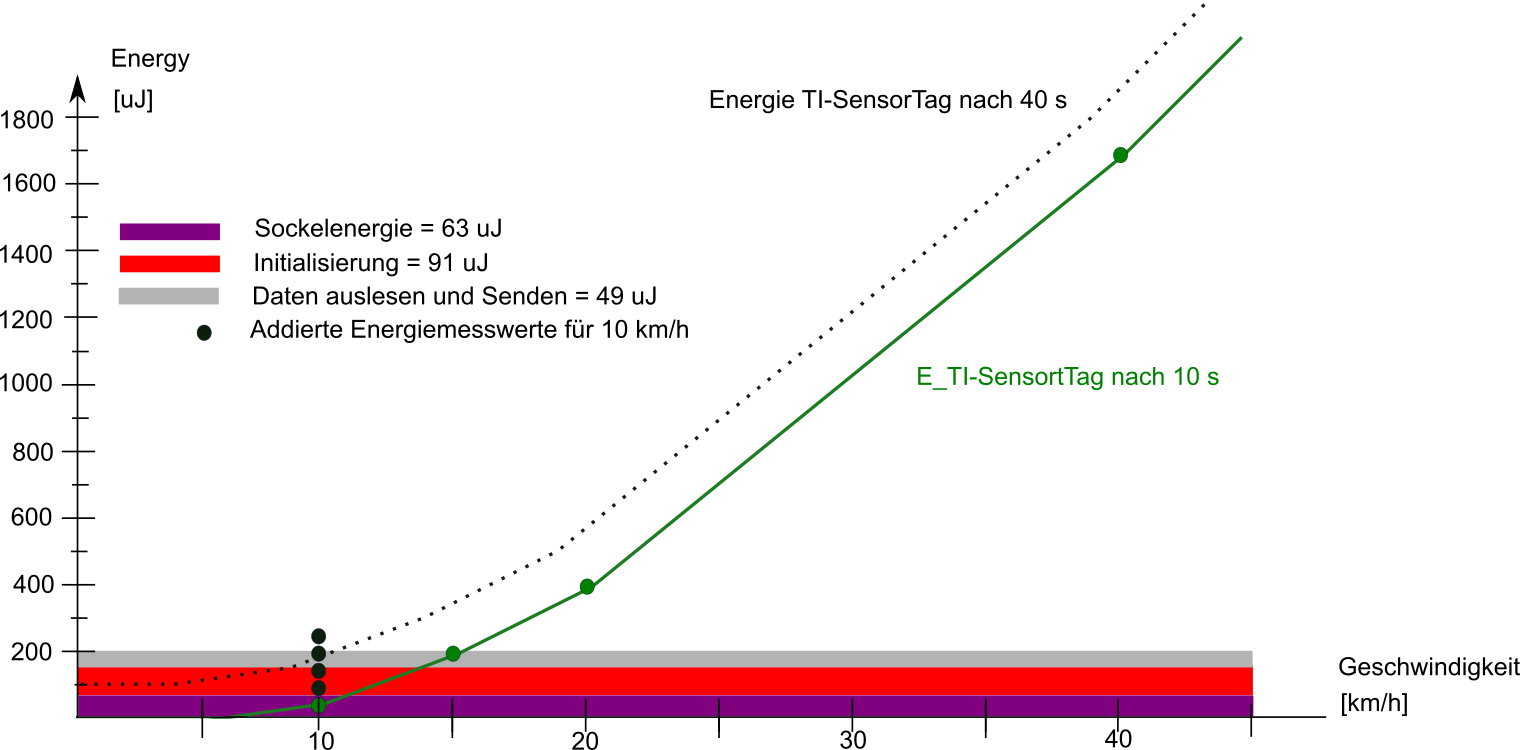
\includegraphics[width=1\textwidth]{4Resultate/imag/EnergyVerbrauchZusammenfassung.png}\label{resultat_Zsm_Energy} 
\caption{Energieverbrauch gem\"{a}ss Verarbeitungsaufwand für CPU}
\end{figure}






\newpage
\section{Ergebnisse BLE-Applikation}

Der Aufbau des TI-SensorTags zusammen mit dem selbst entwickelten Board wird \glqq Sensor\grqq\thinspace\ genannt. Dies, weil aus der Sicht einer Benutzerin oder eines Benutzers keine detaillierte Hardware besteht, sondern \glqq ein Sensor\grqq. Die Vereinfachung dient der Benutzerfreundlichkeit. Die Android-Applikation ist bewusst einfach aufgebaut, um die Benutzerin bzw. den Benutzer nicht zu verwirren. 

Der animierte Tachometer stellt die aktuelle Geschwindigkeit schnell und übersichtlich dar. Weitergehende Funktionen sind durch prägnante Namen selbsterklärend und der User sollte keine Mühe haben, die App ohne Lesen einer Anleitung zu verstehen.

\subsection{Applikationsstruktur}

Beim Öffnen der Applikation wird geprüft, ob Bluetooth aktiviert ist (siehe Abbildung \ref{permission}). Sollte Bluetooth nicht aktiviert sein, wird der User gefragt, ob Bluetooth aktiviert werden darf. Sollte der User die Aktivierung ablehnen schliesst sich die Applikation sofort.

\begin{figure}[ht]
    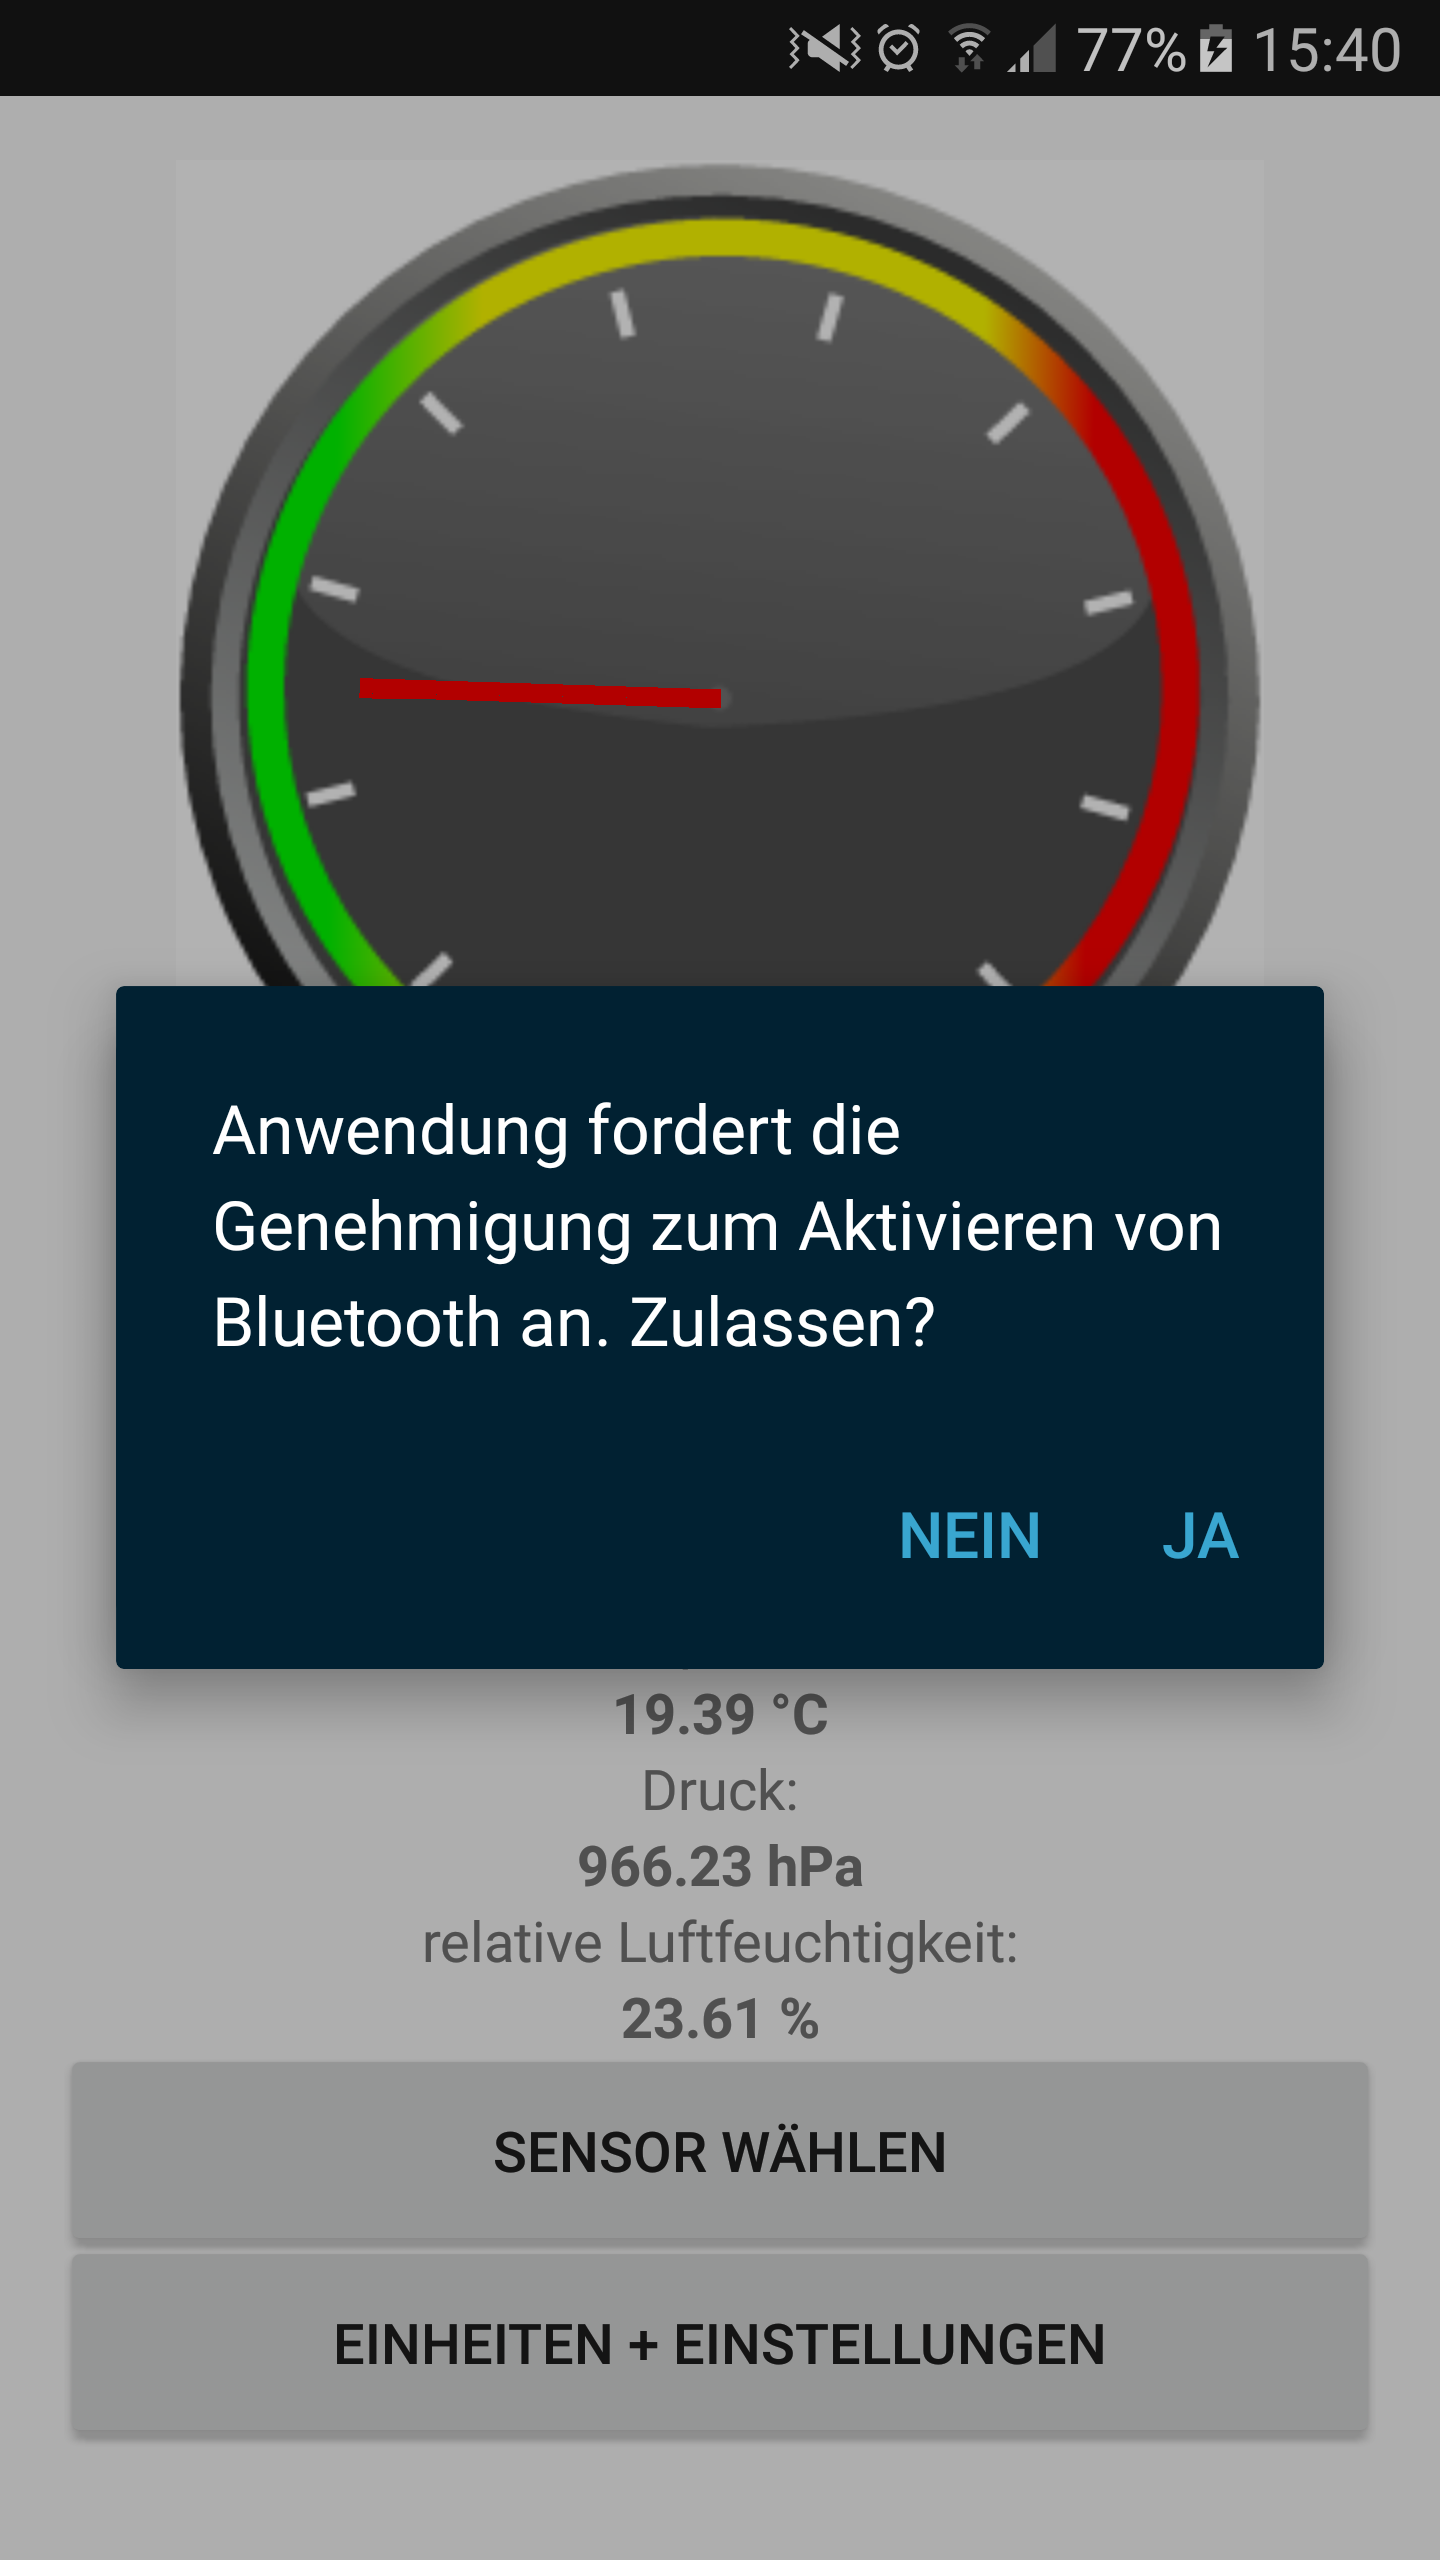
\includegraphics[width=0.5\textwidth]{4Resultate/imag/BLEBluetoothPermission.png} 
    \caption{Bluetooth Permission}
    \label{permission}
\end{figure}

Wird die Aktivierung der Bluetooth-Schnittstelle erlaubt, erscheint der Startbildschirm. Auf diesem befindet sich zentral der Tachometer (siehe Abbildung \ref{tacho}). Dieser zeigt Geschwindigkeiten von 0 – 90 km/h mit einer animierten Tachonadel an. Unterhalb des Tachometers werden die einzelnen Messwerte angezeigt und im untersten Teil des Startbildschirms befinden sich zwei Buttons, über die man Einstellungen vornehmen kann. Die Kontextmenus zu diesen Einstellungen werden in den nächsten zwei Abbildungen \ref{sensorauswahl} und \ref{einheiten} ersichtlich. 

\begin{figure}[ht]
    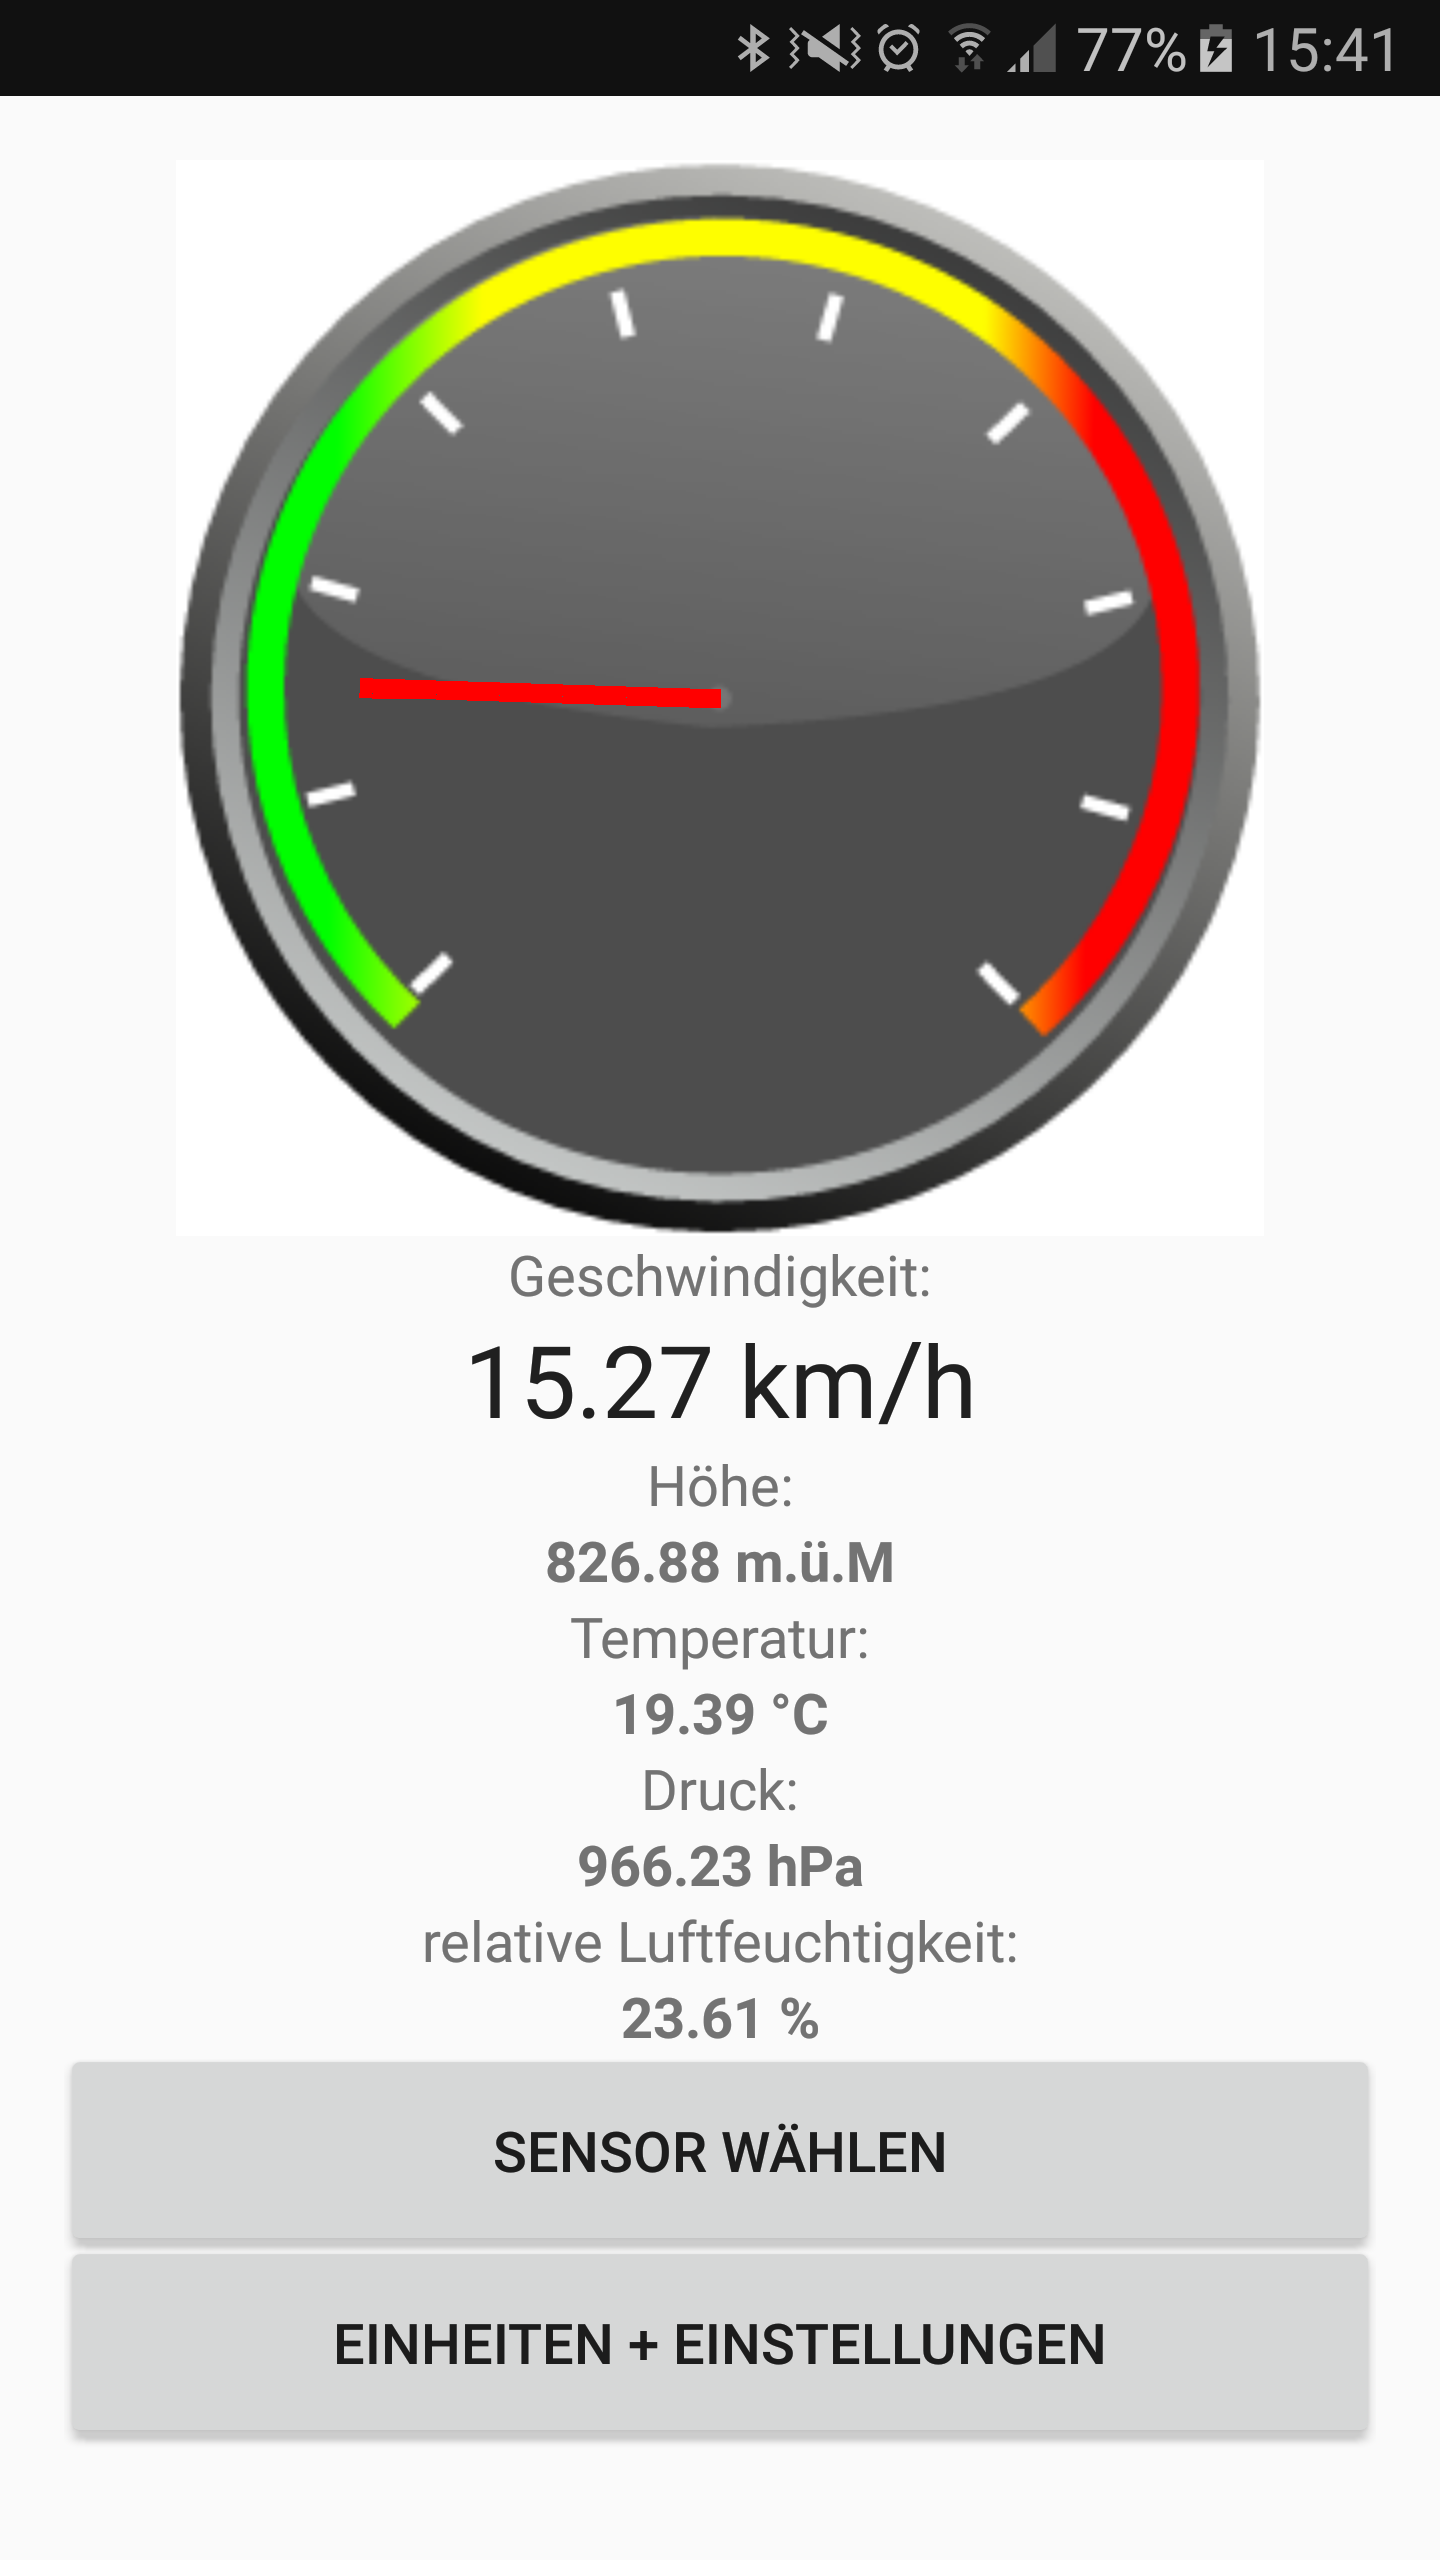
\includegraphics[width=0.5\textwidth]{4Resultate/imag/APPHomeScreen.png} 
    \caption{Startbildschirm der Applikation}
    \label{tacho}
\end{figure}

Wählt man auf dem Startbildschirm \glqq Sensor wählen\grqq, erscheint ein neuer Bildschirm. Auf diesem erscheinen nur die aktiven Bluetooth Geräte mit dem implementierten Prototypen-Filter. Der Bildschirm bildet die TI-SensorTag-Adresse ab. Der Verbund aus unserer neuen Leiterplatte und dem TI-SensorTag wird absichtlich als Sensor betittelt, da es sich für den User um ein Gerät handelt, welches Umgebungsdaten misst. Der User sieht das Gerät nicht in seinen Einzelteilen, sondern nimmt es als einen Sensor war. Es ist natürlich klar, dass nicht der Sensor (Temperatursensor, Drucksensor, etc) auf dem TI-SensorTag an sich ausgewählt wird, sondern die Adresse des Bluetooth-Chips. Jedoch ist das für einen User ohne technischen Hintergrund zu hochstehend. Jedes TI-SensorTag hat eine eigene Adresse und bei mehreren Prototypen im Raum, kann das entsprechende Gerät ausgewählt werden. Es muss noch überlegt werden, wie die Adresse benutzerfreundlicher gestaltet werden kann, da die Adresse nicht sofort mit einem spezifischen TI-SensorTag in Verbindung gebracht werden kann.

\begin{figure}[ht]
    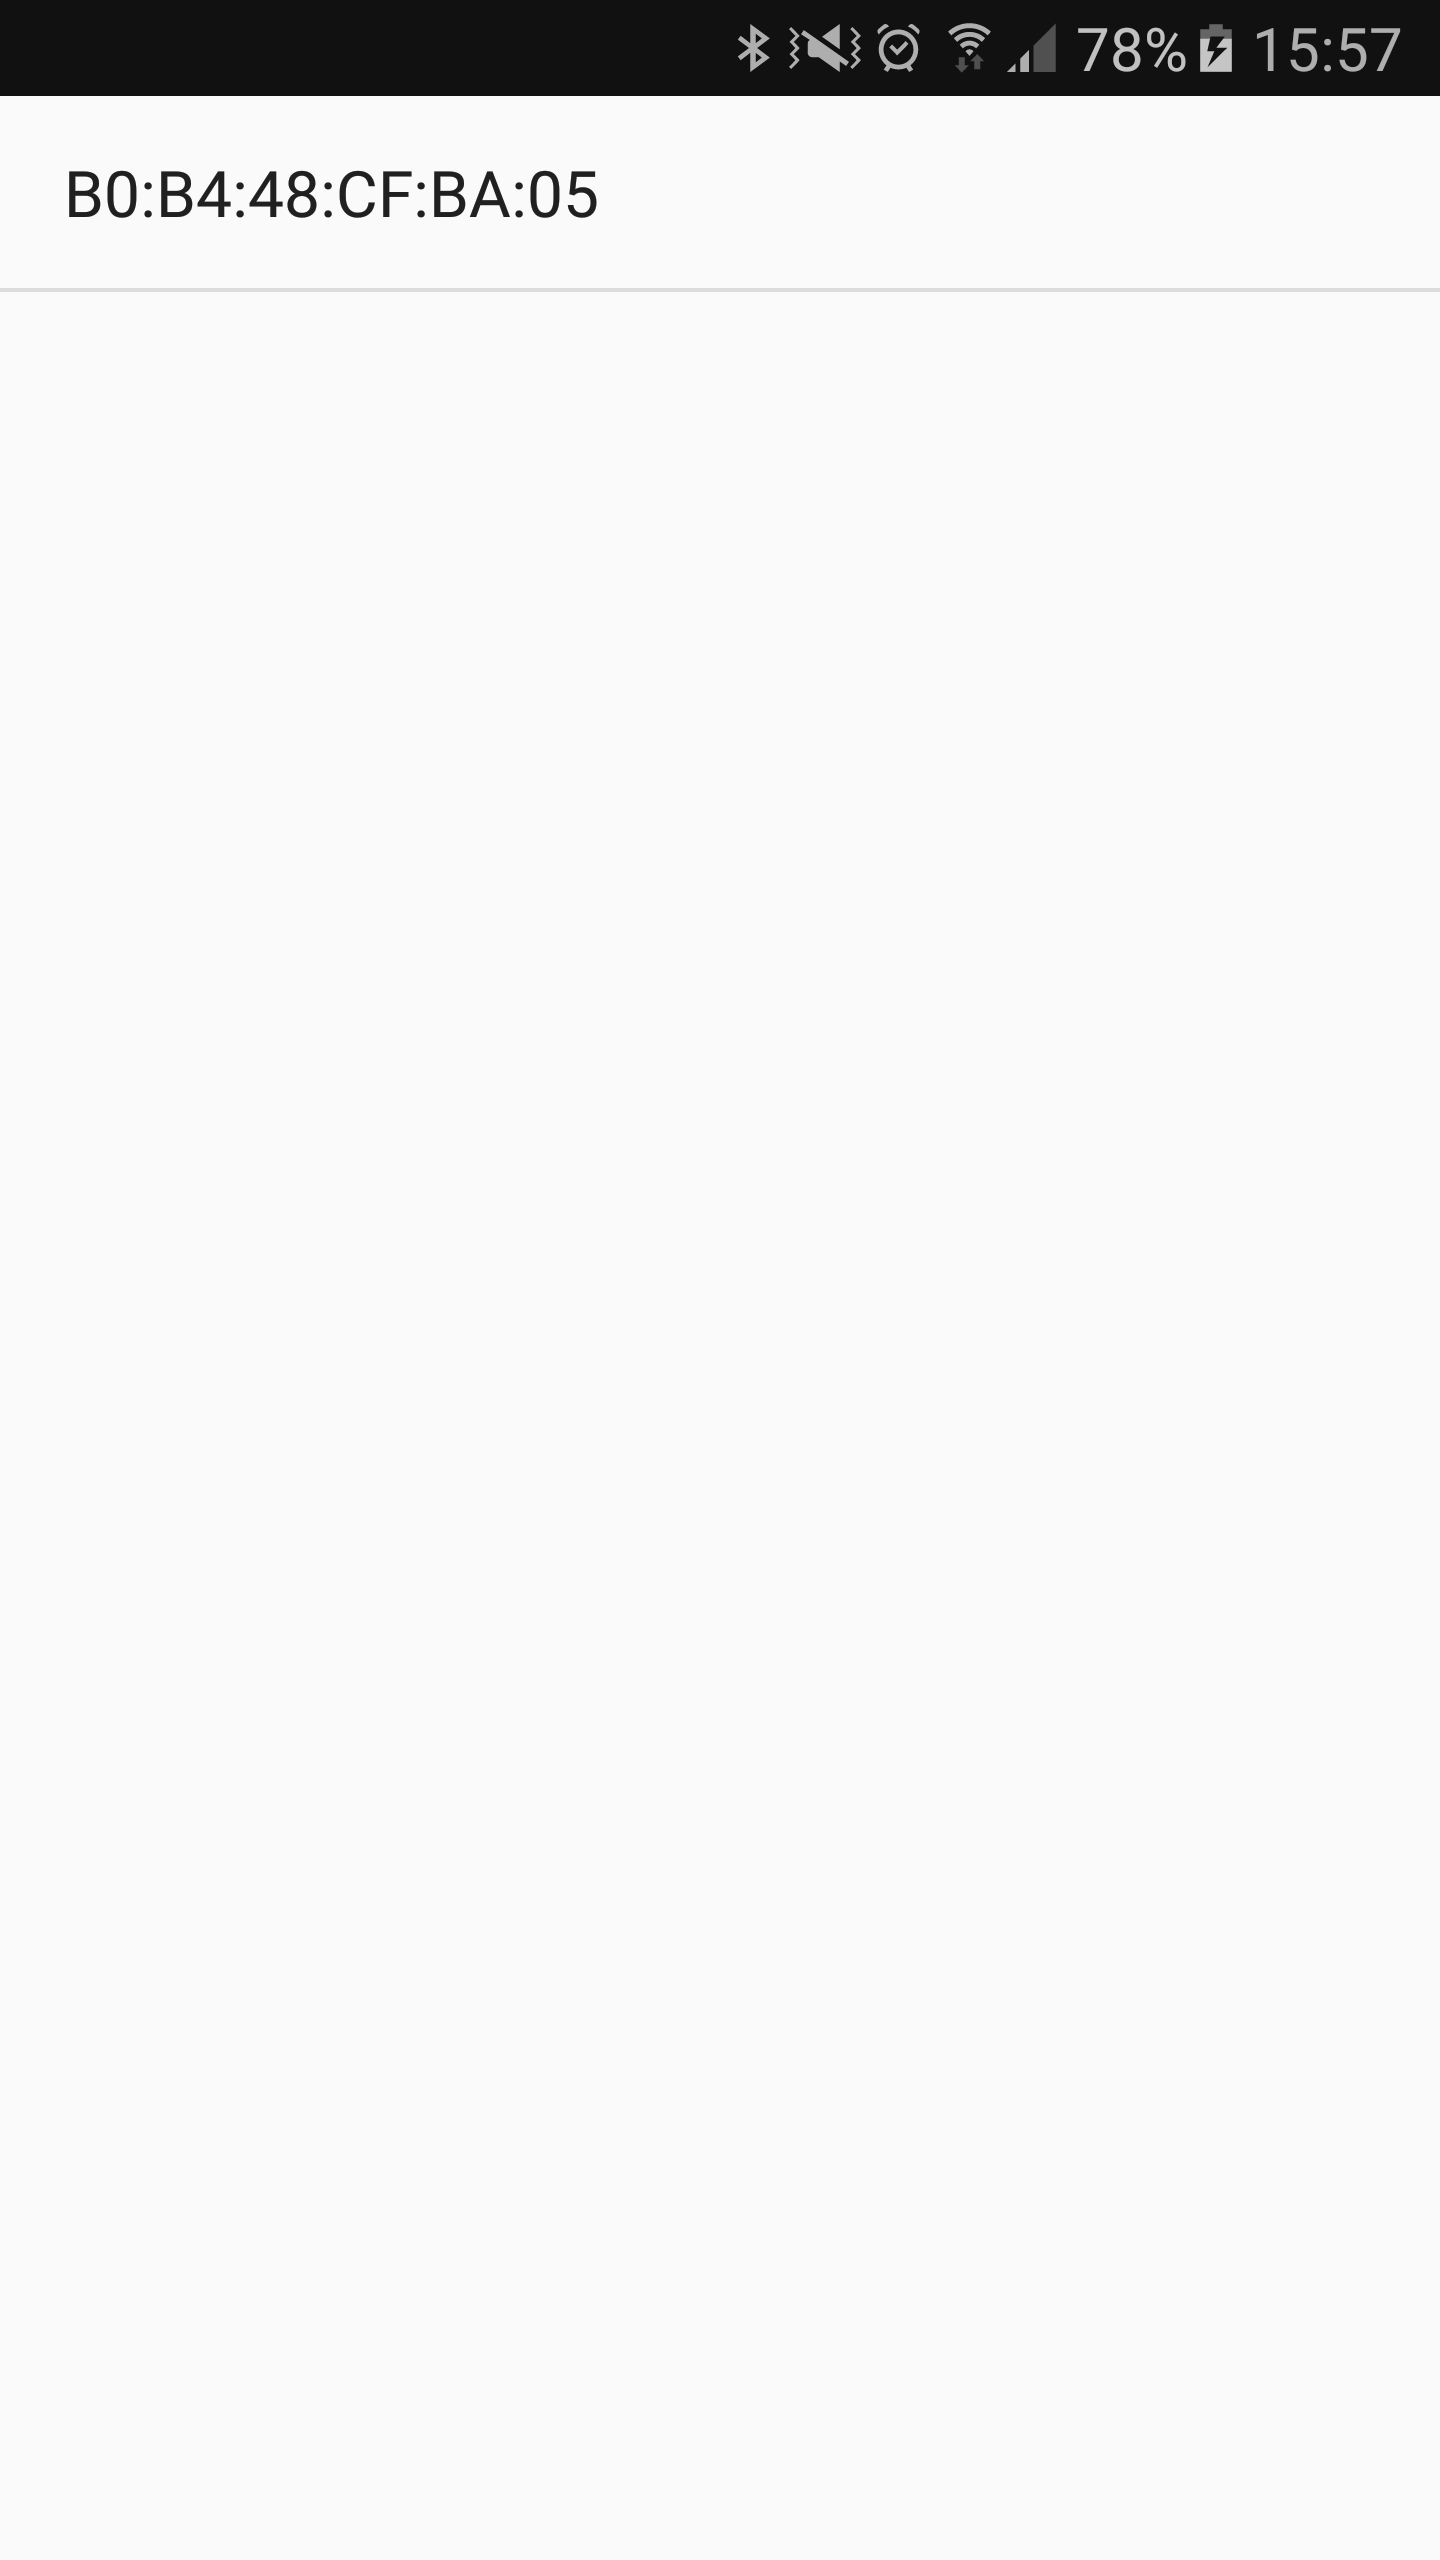
\includegraphics[width=0.5\textwidth]{4Resultate/imag/BLEAdresseAuswaehlen.png} 
    \caption{TI-SensorTagauswahl}
    \label{sensorauswahl}
\end{figure}

Auf dem Startbildschirm befindet sich auch ein Konfigurationsknopf. In das Untermenu gelangt man, in dem man den Button "Einheiten + Einstellungen" auswählt.

\begin{figure}[ht]
    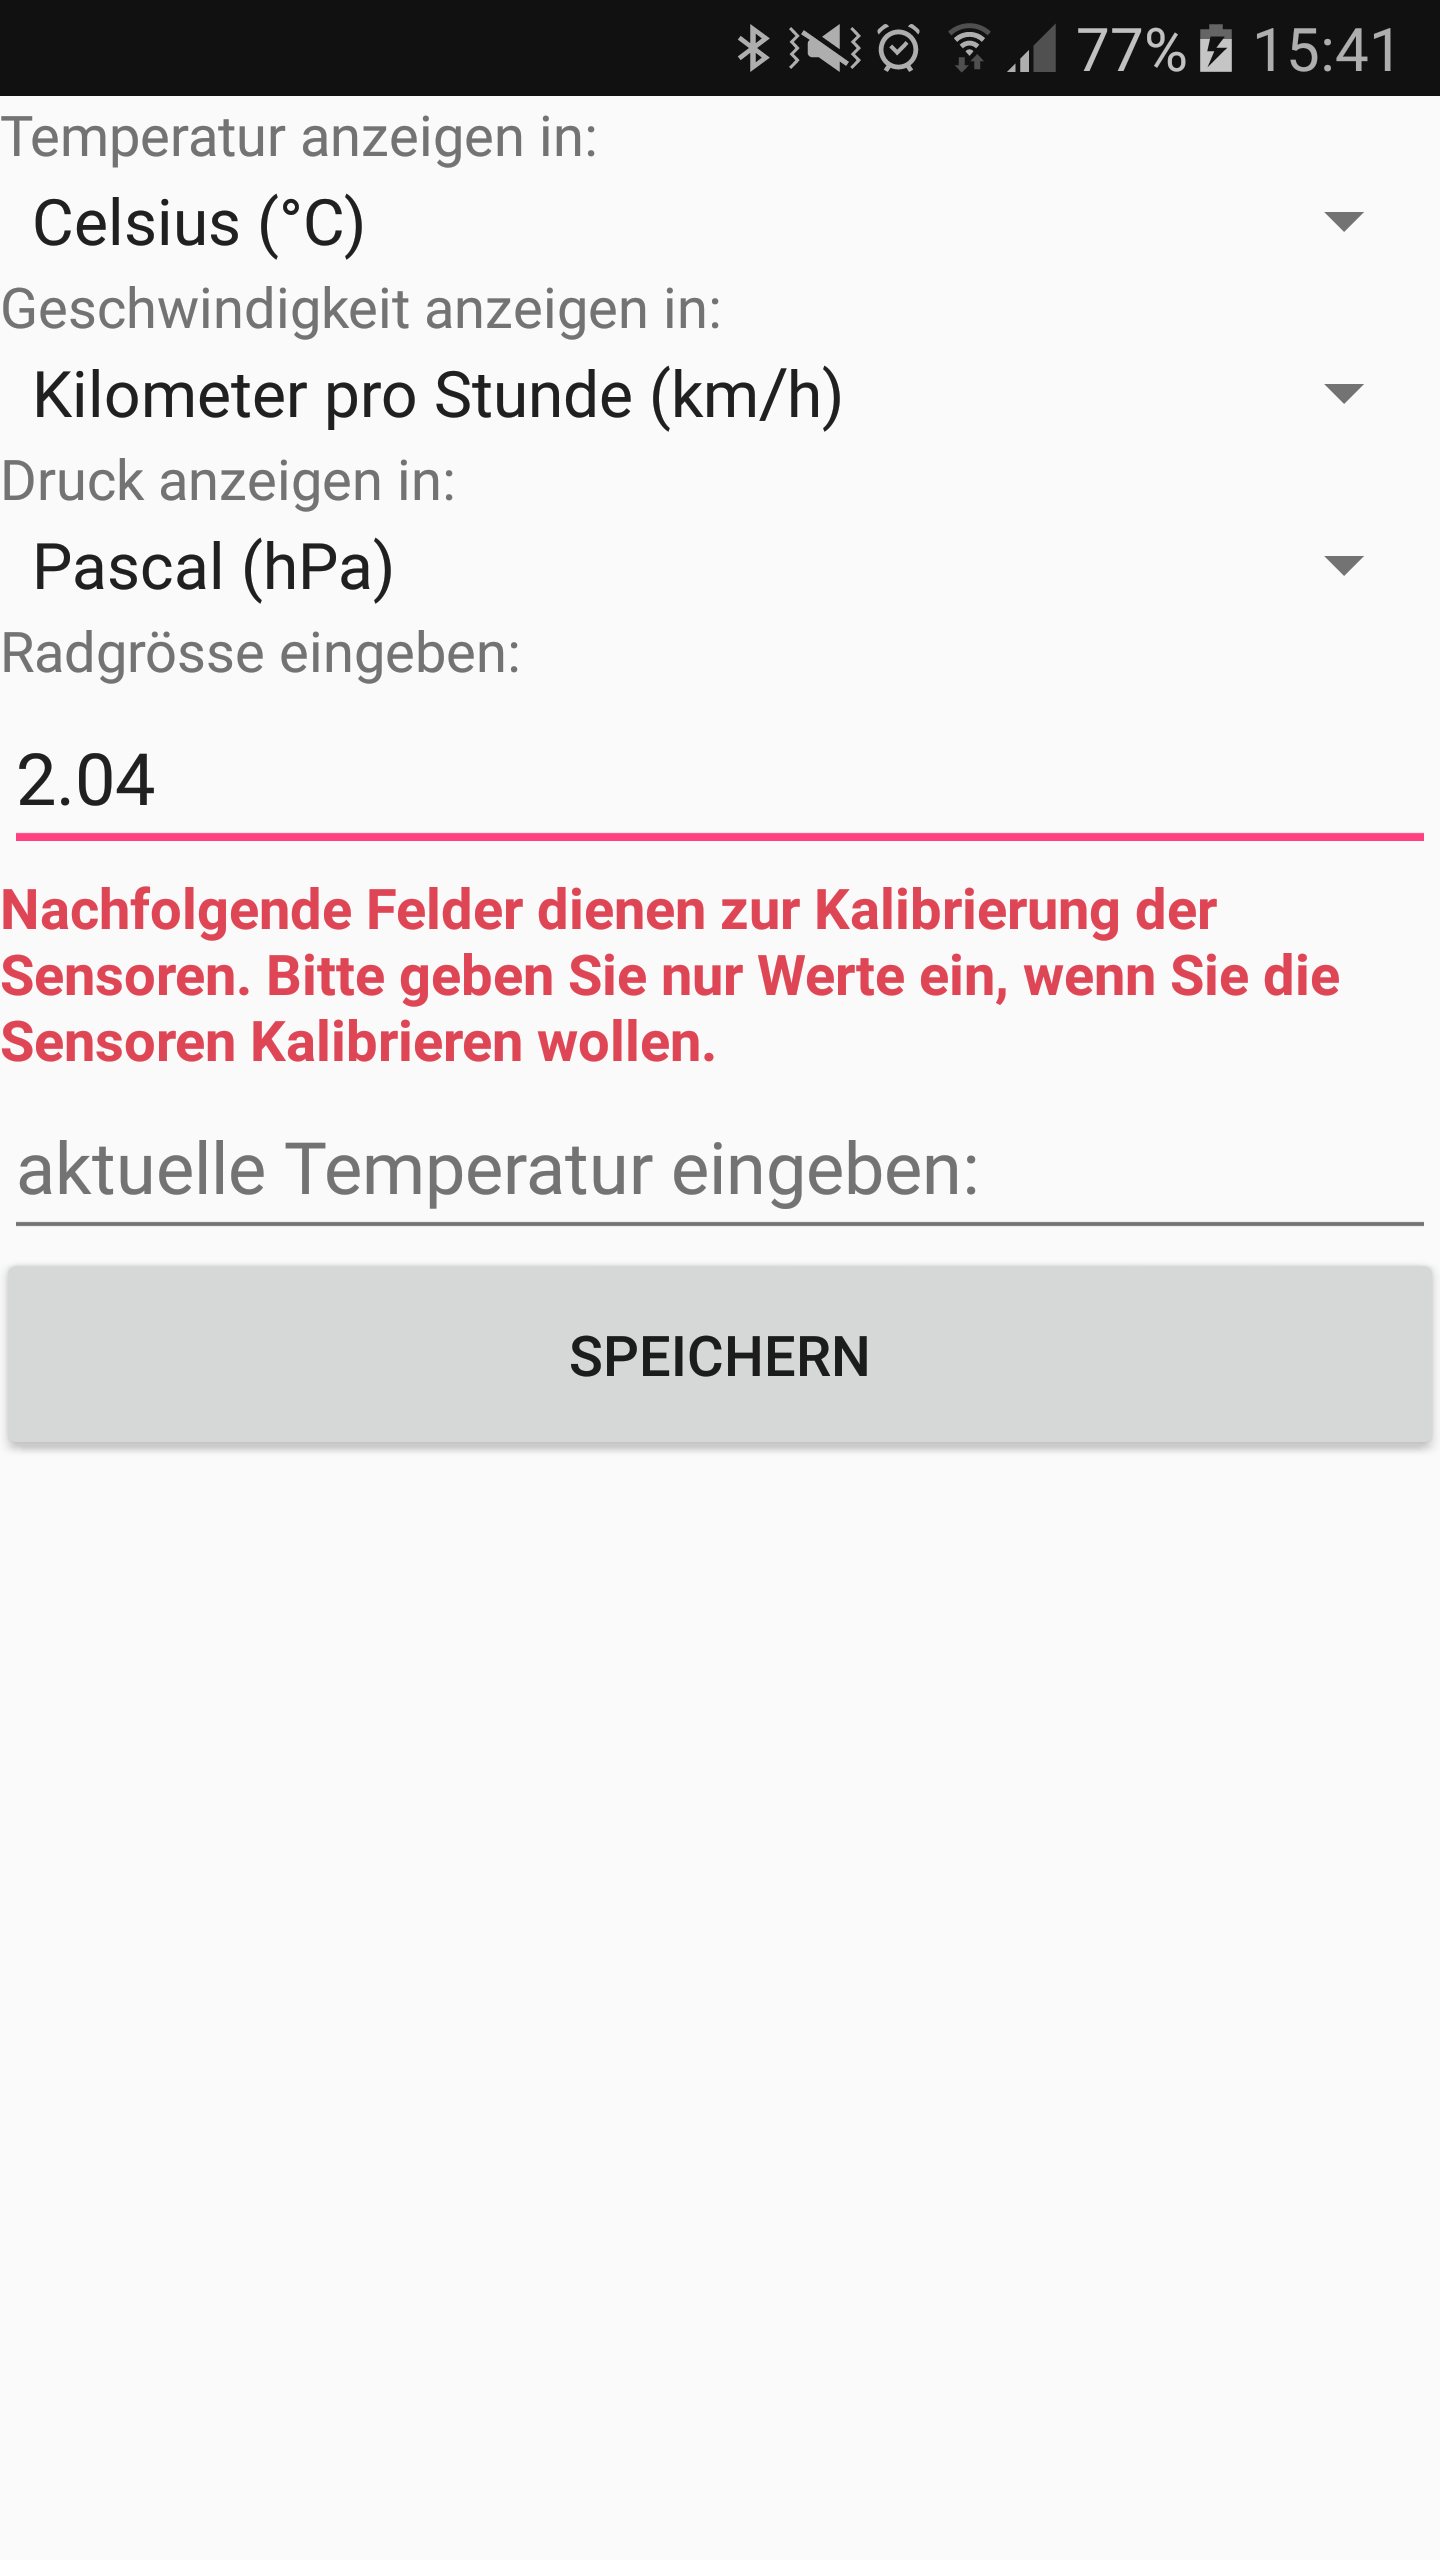
\includegraphics[width=0.5\textwidth]{4Resultate/imag/BLEEinheitenUndEinstellungenStart.png} 
    \caption{Einheiten und Einstellungen}
    \label{einheiten}
\end{figure}

Die Applikation stellt reiche Konfigurationsmöglichkeiten zur Verfügung (siehe Abbildung \ref{einheiten}. Zu jedem Sensor gehört ein Drop Down-Element, in dem die Einheiten ausgewählt werden können. Neben der Einheitenauswahl verfügt die App über die Möglichkeit, den Radumfang anzupassen und die Temperatur zu kalbrieren. 

Die Radgrösse, sprich der Radumfang, muss einstellbar sein, da die interne Geschwindigkeitsberechnung von diesem abhängt. Da die Radgrösse nicht normiert ist, konnte kein Drop Down-Element eingebaut werden. Die Zahl wird über die Tastatur in das Feld eingegeben, es können nur Zahlen eingegeben werden. Dies wurde implementiert um zu verhindern dass die Eingabe von der Applikation nicht interpretiert werden kann.

Bei der Temperaturanzeige ist eine Kalibrierung eingebaut. Dies, weil alle drei Temperatursensoren auf dem TI-SensorTag einheitlich zu hohe Werte ausgeben. Der zu hohe Temperaturwert liegt am Aufbau des Prototypen. TI-SensorTag und Print liegen nahe aufeinander und es entsteht Wärme im Zwischenraum. Der Benutzer oder die Benutzerin kann den korrekten Wert im Kalibrationsfeld eingeben. Die nächste Temperatur, die empfangen wird, wird mit dem eingetragenen Wert verglichen und ein Offset wird eingestellt. Wird keine Kalibration eingetragen, wird die Temperatur nicht kalibriert und der Offset bleibt unverändert.

\subsubsection*{Auswählbare Einheiten}
\begin{tabbing}
    Temperatur     \quad\= Geschwindigkeit            \quad\= Druck \\[0.8ex]
    Celsius (C)    \> Kilometer pro Stunde (km/h)\> Pascal (haP)\\
    Fahrenheit (F) \> Miles per hour (mph)       \> Bar (bar)\\
    Kelvin (K)     \>                            \> Atmosph\"{a}re (atm)\\
                   \>                      \> Pound-Force per sqare inch (psi)\\
                   \>                      \> Millimeter Quecksilber (mmHG)\\
\end{tabbing} 

  
Die vorgenommenen Einstellungen werden über den Button \glqq Speichern\grqq gesichert. Danach werden die eingelesenen Sensordaten in den ausgewählten Einheiten dargestellt.

\subsection{Paketverlust}

TI-SensorTag sendet im Advertising Mode drei Pakete pro Sendevorgang. Gemessen wird der Paketverlust bei einer Geschwindigkeit von 20 km/h (siehe untenstehende Tabelle und \todo{Messprotokoll erwähnen}). \todo{Tabelle referenzieren}  

\subsubsection*{Paketverlust BLE-Applikation}
\begin{tabbing}
    Messperiode \quad\= Gesendete Pakete \quad\= Empfangene Pakete \quad\= Paketverlust\\[0.8ex]
    1 min  \> 38   \> 35 \> 7.9\thinspace\%  \\
    1 min  \> 37   \> 31 \> 16.2\thinspace\%  \\
    2 min  \> 75   \> 64 \> 14.7\thinspace\%  \\
    2 min  \> 77   \> 65 \> 15.6\thinspace\%  \\
    5 min  \> 193   \> 168 \> 13.0\thinspace\%  \\
    5 min  \> 190   \> 158 \> 16.8\thinspace\%  \\
    10 min  \> 345   \> 301 \> 12.8\thinspace\%  \\
    10 min  \> 349   \> 302 \> 13.5\thinspace\%  \\
\end{tabbing} 

Da unsere Nutzung des Advertising Mode keine aktive Verbindung vorsieht, ist ein Paketverlust von rund 15\thinspace\% zu erwarten. Der Paketverlust ist normalerweise keine Problem, da der Empfänger bei feststellen eines Verlusts eine Aufforderung an den Sender schickt um das verlorene Paket neu zu senden. 

\subsection{Korrektheit der Daten}

Die Korrektheit der empfangenen Daten auf der Applikation wird mit einem visuellen Vergleich der Datenpakete im BLE-Sniffer von TI verglichen (siehe Abbildung \ref{sniffer}).  Die Daten im Sniffer entsprechen exakt den Daten, welche die Applikation empfängt. Der Inhalt der Daten wird somit unverfälscht übermittelt.


\todo{aktuelles Sniffer Bild} 

\begin{figure}[ht]
    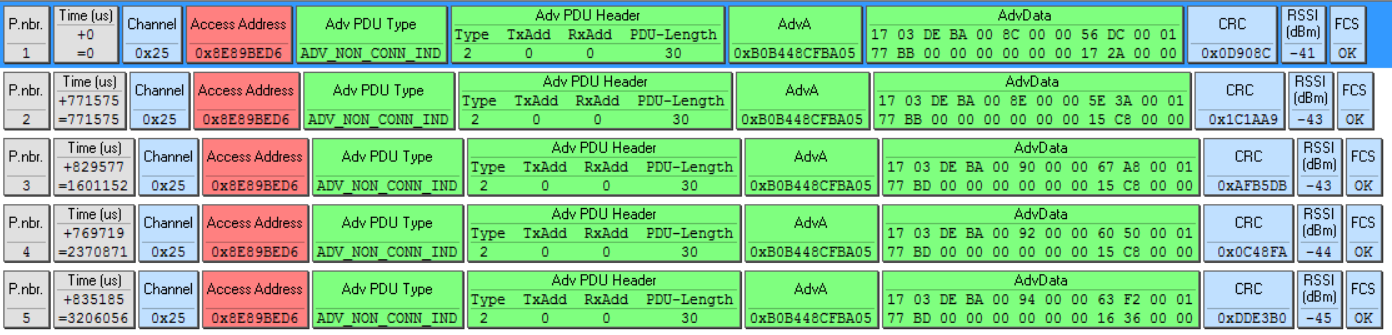
\includegraphics[width=0.5\textwidth]{4Resultate/imag/sniffer.png} 
    \caption{Empfangende Daten des Sniffers}
    \label{sniffer}
\end{figure}

\begin{figure}[ht]
    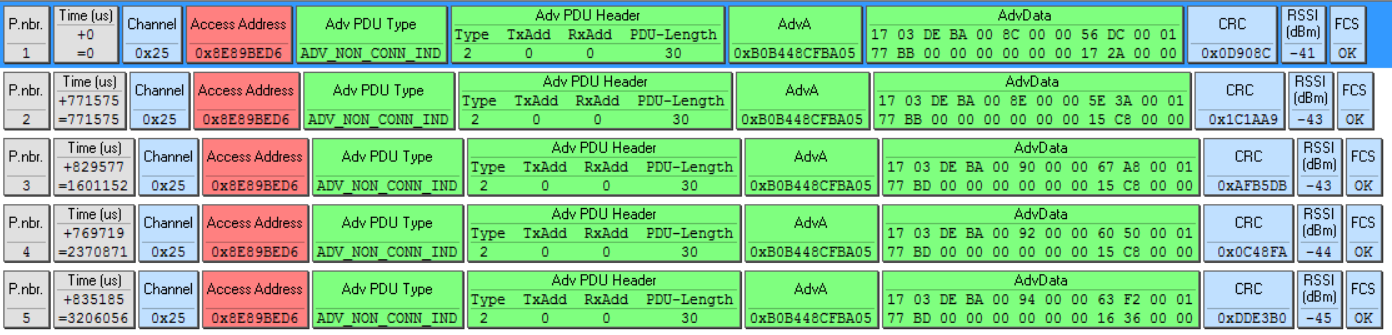
\includegraphics[width=0.5\textwidth]{4Resultate/imag/sniffer.png} 
    \caption{Empfangene Daten der Applikation}
    \label{applikation_daten}
\end{figure}


\todo{Video zeiger (auf CD)}






